\begin{frame}
  \frametitle{\textbf{Jet Suppression and Asymmetry}}
  \begin{columns}
    
    \column{0.5\textwidth}

    \begin{tikzpicture}
      \node{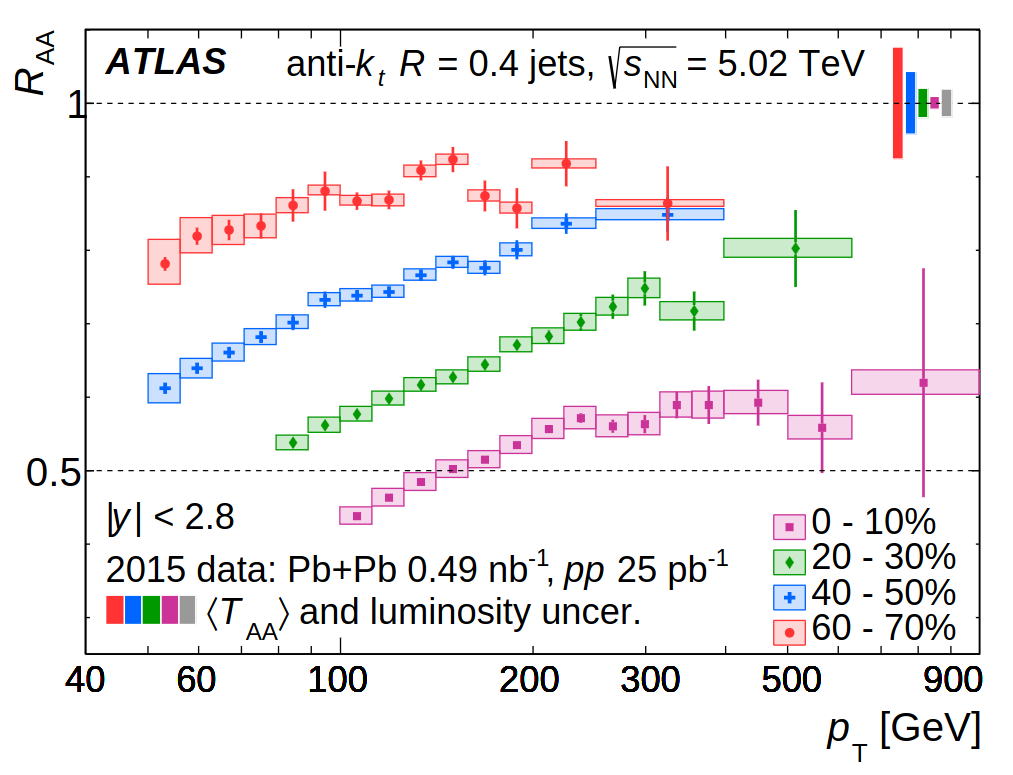
\includegraphics[width=\textwidth]{atlas-jet-raa.png}};
      \node[font=\tiny] at (-1,-2) {\href{https://arxiv.org/abs/1805.05635}{arXiv:1805.05635}};
    \end{tikzpicture}

    \

    
    \begin{tikzpicture}
      \node{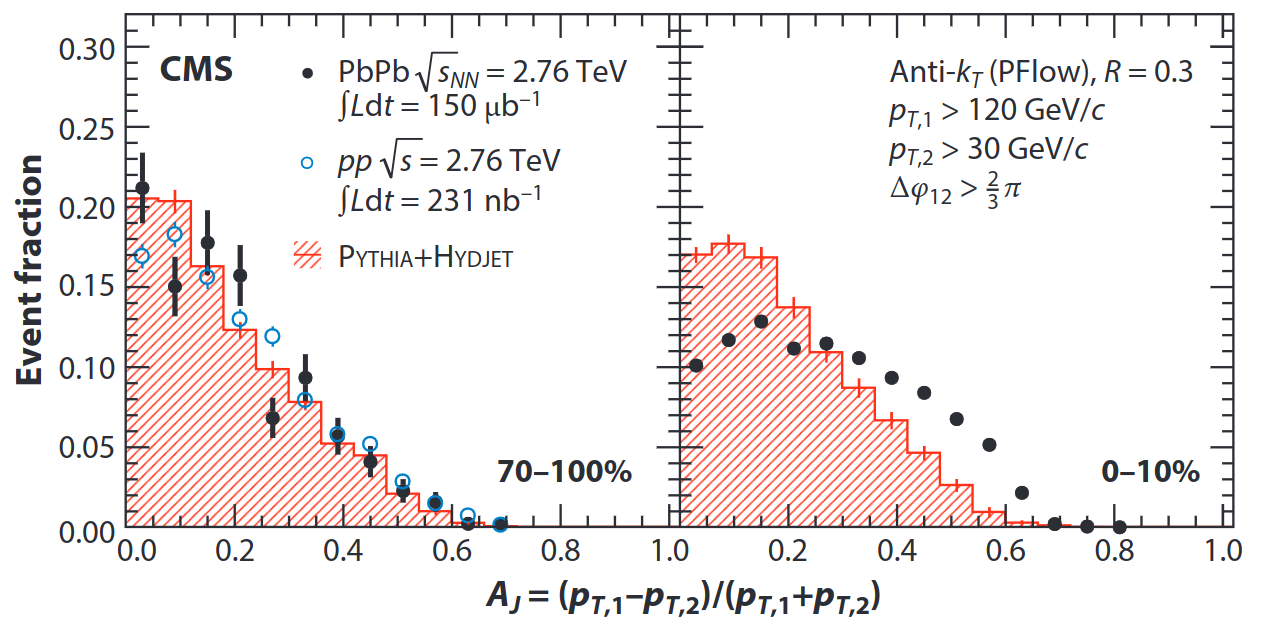
\includegraphics[width=\textwidth]{dijet-asymmetry.png}};
    \end{tikzpicture}

    \column{0.5\textwidth}
    \begin{itemize}
    %\item Fully-reconstructed jets are better probes of medium properties than leading hadrons
    \item Jet $R_{\text{AA}}$: measure of the suppression of jet production in AA collisions as compared to pp collisions
    %\item Fragmenting daughter-partons lose energy via gluon interactions $\to$ lose energy $\to$ final-state jet is ``suppressed''
    \end{itemize}
    \begin{align*}
      R_{\text{AA}}^{\text{jet}} (p_{\text{T}}) = \cfrac{dN^{\text{AA}}_{\text{jet}} / dp_{\text{T}}}{\left< N_{\text{coll}} \right> dN^{\text{pp}}_{\text{jet}} / dp_{\text{T}}}
    \end{align*}
    \begin{itemize}
    \item We expect asymmetric suppression in dijet events, since one jet will interact with more QGP than the other
    \item Quantify via dijet-asymmetry $A_J$
      \begin{align*}
        A_J = \cfrac{p_{\text{T},1} - p_{\text{T},2}}{p_{\text{T},1} + p_{\text{T},2}}
      \end{align*}
    \item Jet suppression \& asymmetry $\to$ \textbf{consistent with presence of QGP}
    \item Not seen in small systems (pp, pPb)
    \end{itemize}
  \end{columns}

\end{frame}
